%%%%%%%%%%%%%%%%%%%%%%%%%%%%%%%%%%%%%%%%%%%%%%%%%%%%%%%%%%%%%%%%%%%%%%
%%  Copyright by Wenliang Du.                                       %%
%%  This work is licensed under the Creative Commons                %%
%%  Attribution-NonCommercial-ShareAlike 4.0 International License. %%
%%  To view a copy of this license, visit                           %%
%%  http://creativecommons.org/licenses/by-nc-sa/4.0/.              %%
%%%%%%%%%%%%%%%%%%%%%%%%%%%%%%%%%%%%%%%%%%%%%%%%%%%%%%%%%%%%%%%%%%%%%%

\newcommand{\commonfolder}{../../common-files}

\documentclass[11pt]{article}

\usepackage[most]{tcolorbox}
\usepackage{times}
\usepackage{epsf}
\usepackage{epsfig}
\usepackage{amsmath, alltt, amssymb, xspace}
\usepackage{wrapfig}
\usepackage{fancyhdr}
\usepackage{url}
\usepackage{verbatim}
\usepackage{fancyvrb}
\usepackage{adjustbox}
\usepackage{listings}
\usepackage{color}
\usepackage{subfigure}
\usepackage{cite}
\usepackage{sidecap}
\usepackage{pifont}
\usepackage{mdframed}
\usepackage{textcomp}
\usepackage{enumitem}


% Horizontal alignment
\topmargin      -0.50in  % distance to headers
\oddsidemargin  0.0in
\evensidemargin 0.0in
\textwidth      6.5in
\textheight     8.9in 

\newcommand{\todo}[1]{
\vspace{0.1in}
\fbox{\parbox{6in}{TODO: #1}}
\vspace{0.1in}
}


\newcommand{\unix}{{\tt Unix}\xspace}
\newcommand{\linux}{{\tt Linux}\xspace}
\newcommand{\minix}{{\tt Minix}\xspace}
\newcommand{\ubuntu}{{\tt Ubuntu}\xspace}
\newcommand{\setuid}{{\tt Set-UID}\xspace}
\newcommand{\openssl} {\texttt{openssl}}


\pagestyle{fancy}
\lhead{\bfseries SEED Labs}
\chead{}
\rhead{\small \thepage}
\lfoot{}
\cfoot{}
\rfoot{}


\definecolor{dkgreen}{rgb}{0,0.6,0}
\definecolor{gray}{rgb}{0.5,0.5,0.5}
\definecolor{mauve}{rgb}{0.58,0,0.82}
\definecolor{lightgray}{gray}{0.90}


\lstset{%
  frame=none,
  language=,
  backgroundcolor=\color{lightgray},
  aboveskip=3mm,
  belowskip=3mm,
  showstringspaces=false,
%  columns=flexible,
  basicstyle={\small\ttfamily},
  numbers=none,
  numberstyle=\tiny\color{gray},
  keywordstyle=\color{blue},
  commentstyle=\color{dkgreen},
  stringstyle=\color{mauve},
  breaklines=true,
  breakatwhitespace=true,
  tabsize=3,
  columns=fullflexible,
  keepspaces=true,
  escapeinside={(*@}{@*)}
}

\newcommand{\newnote}[1]{
\vspace{0.1in}
\noindent
\fbox{\parbox{1.0\textwidth}{\textbf{Note:} #1}}
%\vspace{0.1in}
}


%% Submission
\newcommand{\seedsubmission}{You need to submit a detailed lab report, with screenshots,
to describe what you have done and what you have observed.
You also need to provide explanation
to the observations that are interesting or surprising.
Please also list the important code snippets followed by
explanation. Simply attaching code without any explanation will not
receive credits.}

%% Book
\newcommand{\seedbook}{\textit{Computer \& Internet Security: A Hands-on Approach}, 2nd
Edition, by Wenliang Du. See details at \url{https://www.handsonsecurity.net}.}

%% Videos
\newcommand{\seedisvideo}{\textit{Internet Security: A Hands-on Approach},
by Wenliang Du. See details at \url{https://www.handsonsecurity.net/video.html}.}

\newcommand{\seedcsvideo}{\textit{Computer Security: A Hands-on Approach},
by Wenliang Du. See details at \url{https://www.handsonsecurity.net/video.html}.}

%% Lab Environment
\newcommand{\seedenvironment}{This lab has been tested on our pre-built
Ubuntu 16.04 VM, which can be downloaded from the SEED website. }

\newcommand{\seedenvironmentA}{This lab has been tested on our pre-built
Ubuntu 16.04 VM, which can be downloaded from the SEED website. }

\newcommand{\seedenvironmentB}{This lab has been tested on our pre-built
Ubuntu 20.04 VM, which can be downloaded from the SEED website. }

\newcommand{\seedenvironmentAB}{This lab has been tested on our pre-built
Ubuntu 16.04 and 20.04 VMs, which can be downloaded from the SEED website. }

\newcommand{\nodependency}{Since we use containers to set up the lab environment, 
this lab does not depend too much on our SEED VM. You can do this lab
using other VMs or physical machines. }







\newcommand{\seedlabcopyright}[1]{
\vspace{0.1in}
\fbox{\parbox{6in}{\small Copyright \copyright\ {#1}\ \ by Wenliang Du.\\
      This work is licensed under a Creative Commons
      Attribution-NonCommercial-ShareAlike 4.0 International License.
      If you remix, transform, or build upon the material, 
      this copyright notice must be left intact, or reproduced in a way that is reasonable to
      the medium in which the work is being re-published.}}
\vspace{0.1in}
}






\newcommand{\dnsFigs}{../DNS_in_a_Box/Figs}
\lhead{\bfseries SEED Labs -- DNSSEC Lab}


\def \code#1 {\fbox{\scriptsize{\texttt{#1}}}}

\newcommand{\bankcom}{\url{bank32.com}\xspace}
\newcommand{\wwwbank}{\url{www.bank32.com}\xspace}
\newcommand{\examplenet}{\url{example.net}\xspace}
\newcommand{\wwwexample}{\url{www.example.net}\xspace}
\newcommand{\apollo}{\texttt{Apollo}\xspace}

\begin{document}

\begin{center}
{\LARGE DNS Security Extensions (DNSSEC) Lab}
\end{center}

\seedlabcopyright{2020}


% *******************************************
% SECTION
% ******************************************* 
\section{Lab Overview}

To protect DNS, the Domain Name System
Security Extensions~(DNSSEC) were developed. DNSSEC is a set of extension to
DNS, aiming to provide authentication and integrity checking on DNS data.
With DNSSEC, all answers from DNSSEC
protected zones are digitally signed.  By checking the digital signature, a
DNS resolver is able to check if the information is authentic or not.
With such a mechanism, the DNS cache
poisoning attack will be defeated, because any fake data, whether from a
spoofed response packet or from an authoritative nameserver, will be
detected because they will fail the signature checking.


To help students understand how DNSSEC works, we will
enhance the miniature DNS system developed 
in the DNS-in-a-Box lab with DNSSEC. Students will
configure each of the nameservers, so they all support 
DNSSEC. This lab covers the following topics:

\begin{itemize}[noitemsep]
\item DNS and how it works
\item DNSSEC and how it works
\item Key management, public key, digital signature 
\item Docker container, docker compose
\end{itemize}


\paragraph{Readings and videos.}
Detailed coverage of the DNS protocol and attacks can be found in the following:

\begin{itemize}
\item Chapter 18 of the SEED Book, \seedbook
\item Section 7 of the SEED Lecture, \seedisvideo
\end{itemize}


\paragraph{Lab environment.} 
\seedenvironmentB
\nodependency




% *******************************************
% SECTION
% *******************************************
\section{Lab Environment Setup} 


This lab depends on the DNS-In-a-Box lab, 
so students should do that lab first. After doing the lab,
we will have a miniature DNS system depicted in 
Figure~\ref{dnssec:fig:dns-in-a-box}. In this lab, we will
enhance this infrastructure with DNSSEC. 
In this lab description, we assume that the miniature DNS system 
has already been set up
correctly, and each nameserver is hosted inside a container. 
We will modify each of the container, so the nameserver inside 
can support DNSSEC. Please download the \texttt{Labsetup.zip}
file from the website of this lab (this file is slightly different 
from one used in the DNS-In-a-Box lab).


\begin{figure}[htb]
\begin{center}
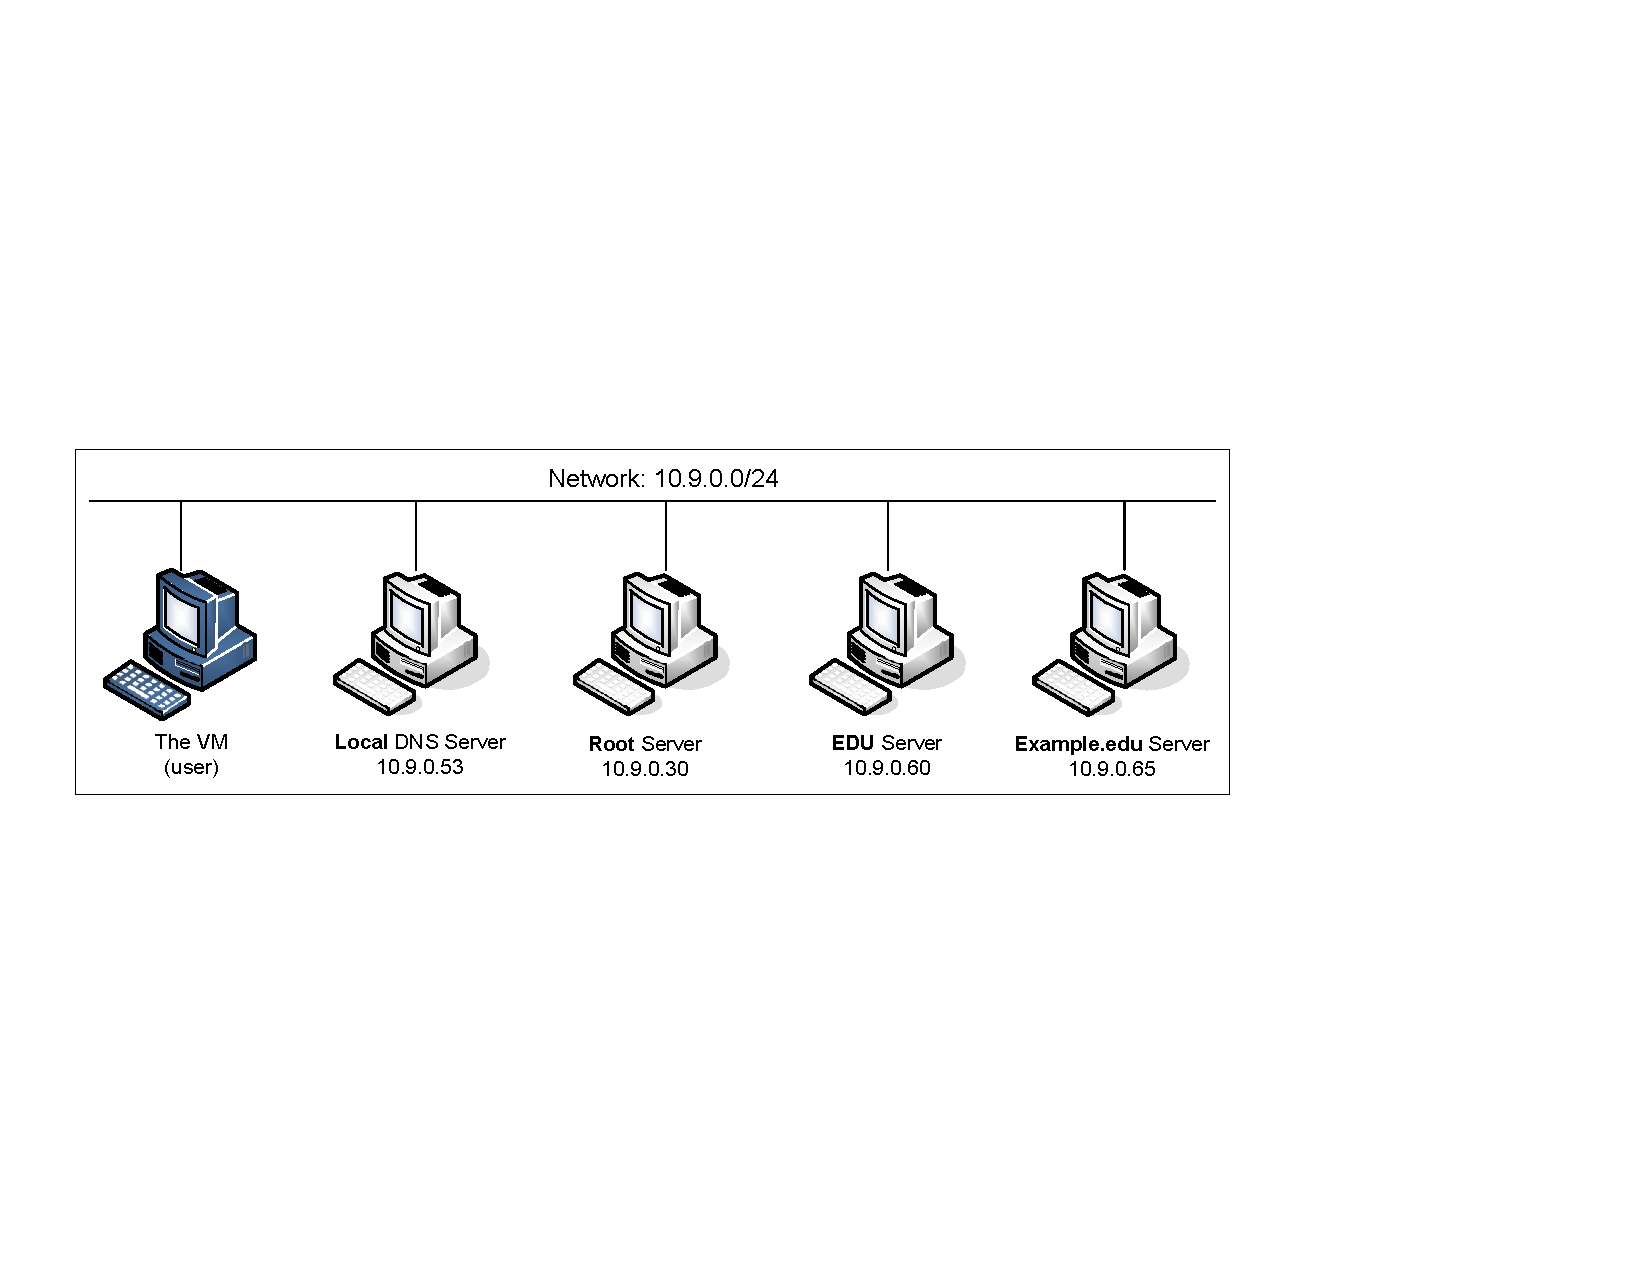
\includegraphics[width=0.95\textwidth]{\dnsFigs/DNS-in-a-box.pdf}
\end{center}
\caption{Lab environment setup}
\label{dnssec:fig:dns-in-a-box}
\end{figure}
 


\paragraph{Software installation.} We will use some tools that 
have not been installed in the SEED VM. Please use the following
command to install the software: 

\begin{lstlisting}
$ sudo apt-get install bind9utils
\end{lstlisting}
 


% *******************************************
% SECTION
% ******************************************* 
\section{Task 1: Set up the \texttt{example.edu} Domain}


In this task, we will go to the container folder for the 
\texttt{example.edu} nameserver. This container, built 
from the DNS-in-a-Box lab, hosts 
the \texttt{example.edu} domain. 
We will modify the files inside this folder, so the nameserver
can support DNSSEC queries. 



% -------------------------------------------
% SUBSECTION
% ------------------------------------------- 
\subsection{Task 1.a: Enabling DNSSEC}

To enable DNSSEC on this server, we need to add the following entry to the 
configuration file \path{named.conf.options}. Please check the settings
in the lab setup file to ensure this is set. 

\begin{lstlisting}
dnssec-enable yes;
dnssec-validation auto;
\end{lstlisting}



% -------------------------------------------
% SUBSECTION
% ------------------------------------------- 
\subsection{Task 1.b: Generating keys for \texttt{example.edu} server} 

First, we need to generate two pairs of keys, one is called Zone Signing Key (ZSK), and 
the other is called Key Signing Key (KSK). Each key consists of a public key and a private key.
ZSK is used to sign the zone records, while the KSK is used to sign the ZSK. 

This two-key scheme is quite common in key management. The one that actually signs the record
(i.e., ZSK) can change frequently to achieve better security. If only one key is used,
when this key changes, the data stored in the key management system needs to be updated. 
In DNSSEC, the parent zone stores the information about this key, so the parent zone file
needs to be updated. 

To avoid this overhead, the second key is introduced. This key is called 
Key Signing Key, i.e., it only signs the ZSK record in the zone file, while the 
other records are still signed by ZSK. The KSK's information is provided to 
the parent zone, but KSK does not change very frequently. When ZSK changes,
all we need to do is to use the KSK to generate a new signature for the ZSK. 

Both ZSK and KSK are public key pairs, but since their roles and lifetime are different,
typically the KSK key is set to be stronger than the ZSK key, i.e., the key size 
is longer. In the following, the first command generates a ZSK key using the 
\texttt{RSASHA256} algorithm with key size being 1024. The second command 
generates a KSK key using the same algorithm, but doubling the key size. 
If the OS cannot find the command, you forgot to 
install the required software (see the lab setup section).


\begin{lstlisting}
dnssec-keygen -a RSASHA256 -b 1024 example.edu
dnssec-keygen -a RSASHA256 -b 2048 -f KSK example.edu
\end{lstlisting}

The second command generate a KSK. The \texttt{-f} option 
put \texttt{257} in the key file, indicating this is the KSK. 
Without this option, a default value \texttt{256} is put in
the key file, indicating this is the ZSK.





% -------------------------------------------
% SUBSECTION
% ------------------------------------------- 
\subsection{Task 1.c: Signing the \texttt{example.edu} domain's zone file} 

We will sign the zone file. This zone file 
is the same as the one used in the DNS-in-a-Box lab. We use the 
following \texttt{dnssec-signzone} command to sign the zone file.  


\begin{lstlisting}
dnssec-signzone -S -o example.edu example.edu.db
\end{lstlisting}
 
With the \texttt{-S} option, the command will look
for the zone signing key and key signing key 
from the specified folder using the zone name (we did not specify the key folder 
using the \texttt{-K} option, so the default is the current folder)
If you have multiple pairs of keys in the specified folder,
the command will generate signatures using each key, so you would get 
multiple signatures for each record. 


Once the zone file is signed, a new zone file ended with
\texttt{.signed} will be generated. Take a look at the file and describe 
what new entries are added to the original zone file. Please explain
their purposes. 


This new zone file will be used by our nameserver, so 
we will modify the \texttt{named.conf.seedlabs} file to tell the 
nameserver to use this file as its zone file. See the following 
example: 

\begin{lstlisting}
zone "example.edu" {
        type master;
        file "/etc/bind/example.edu.db.signed";
};
\end{lstlisting}


% -------------------------------------------
% SUBSECTION
% ------------------------------------------- 
\subsection{Task 1.d: Testing the server}

Using the docker-compose command, we can build and start all the 
containers. We then use the following \texttt{dig} command to conduct the testing. 
The command allows us to directly ask 
a server (\texttt{@server}) to get a specific \texttt{type}
of DNS record for a specific domain or host \texttt{name}.
By using the \texttt{+dnssec} flag, we set the DNSSEC OK bit (DO) in the OPT record 
in the additional section of the query, requesting the server to
send back the related DNSSEC records, such as the signature. 

\begin{lstlisting}
General format:
$ dig @server name type +dnssec

Example:
$ dig @10.9.0.65 example.edu DNSKEY +dnssec
\end{lstlisting}
 

Run the following commands to get different types of records 
from the \texttt{example.edu} nameserver. Provide an explanation
for each of the records in the response. 
In our setup, \texttt{10.9.0.65} is the IP address 
assigned to the \texttt{example.edu} nameserver.

\begin{lstlisting}
$ dig @10.9.0.65 example.edu DNSKEY +dnssec
$ dig @10.9.0.65 example.edu NS +dnssec
$ dig @10.9.0.65 www.example.edu A +dnssec
\end{lstlisting}
 


% *******************************************
% SECTION
% ******************************************* 
\section{Task 3: Setting Up the \texttt{edu} Server}


In this task, we will set up the \texttt{edu} server. 
The instructions are similar to those in Task 1, so we will not repeat them. 


% -------------------------------------------
% SUBSECTION
% ------------------------------------------- 
\subsection{Task 3.a: Finding and understanding the DS record}


After signing the zone file of \texttt{example.edu}, a DS record is generated for the Key
Signing Key, and by default, it is placed inside a file called \texttt{dsset-<xyz>}, where
\texttt{<xyz>} is the zone name. In our case, \texttt{dsset-example.edu.} is the file name.


DS (Delegation Signer) record holds the name of a delegated zone. It 
references a DNSKEY record in the sub-delegated zone. 
The DS record should be placed in the parent zone along with the delegating NS records.
The following gives an example of the DS record:


\begin{lstlisting}
example.edu.   IN DS 10246   8  2   (*@\textbf{563D...(omitted)...1D59D1}@*)
                       (*@\ding{192}@*)              (*@\ding{193}@*)
\end{lstlisting}

A DS record contains a key tag (marked as \ding{192}), which is a 
short numeric value identifying the referenced key. This key
is the Key Signing Key (KSK) for the domain.
The most important element in a DS record is the digest (marked by \ding{193}),
which is the one-way hash value of the KSK. By putting this digest
value in the parent zone (i.e., the \texttt{edu} zone), 
the integrity of the sub-delegated zone's
KSK can be verified. That is the main purpose of this DS record. 



% -------------------------------------------
% SUBSECTION
% ------------------------------------------- 
\subsection{Task 3.b: Setting up the \texttt{edu} server} 

Follow the instruction in Task 1 to set up the configuration 
file and generate the ZSK and KSK keys 
for this domain, and then use the keys to sign
the zone file. The zone file is similar to that used 
in the DNS-in-a-Box lab, but we need to add one more 
entry to the zone file before signing it. 


The entry is the DS record of the sub-delegated zone. 
In our case, the \texttt{example.edu} zone is delegated to 
another nameserver, so the digest of its Key Signing Key must 
be included in the \texttt{edu} zone, so the 
integrity of the key can be verified. 


We can copy and paste the content of the DS record to 
\texttt{edu}'s zone file, or use the following
\texttt{INCLUDE} entry to include the file. The latter 
method is more convenient for the lab, because even if we 
change the Key Signing Key of a zone, the DS record's file name stays the same,
so there is no need to change the parent's zone file.

\begin{lstlisting}
$INCLUDE ../edu.example/dsset-example.edu.
\end{lstlisting}
 



% -------------------------------------------
% SUBSECTION
% -------------------------------------------
\subsection{Task 3.c: Testing} 

Build and run all the containers. Then
run the following commands to get different types of records
from the \texttt{edu} nameserver. Provide an explanation
for each of the records in the response. 
In our setup, \texttt{10.9.0.60} is the IP address 
assigned to the \texttt{edu} nameserver.


\begin{lstlisting}
$ dig @10.9.0.60 edu DNSKEY +dnssec
$ dig @10.9.0.60 edu NS +dnssec
$ dig @10.9.0.60 example.edu +dnssec
\end{lstlisting}




% *******************************************
% SECTION
% *******************************************
\section{Task 4: Setting up the root server} 

The procedure to set up the root server is the same as that in the 
previous task. Remember to add the \texttt{edu} zone's DS record 
to the zone file, before signing the zone.  


\paragraph{Testing.}
Run the following commands to get different types of records
from the \texttt{edu} nameserver. Provide an explanation
for each of the records in the response. In our setup,
\texttt{10.9.0.30} is the 
IP address assigned to the root nameserver.


\begin{lstlisting}
$ dig @10.9.0.30 . DNSKEY +dnssec
$ dig @10.9.0.30 . NS +dnssec
$ dig @10.9.0.30 edu +dnssec
$ dig @10.9.0.30 example.edu +dnssec
\end{lstlisting}




% *******************************************
% SECTION
% *******************************************
\section{Task 5: Setting up the Local DNS Server} 


When a computer needs to resolve the IP address from a hostname (or vice versa),
it sends a request to its helper, which is called local DNS server (it
does not need to be local).  This local DNS server will conduct the
entire DNS resolution process, and then send the result back to the computer.
Please follow the DNS-in-a-Box lab to set up this local DNS server, and also
follow Task 1.a to enable DNSSEC on this server. 

In DNSSEC, each nameserver provides its own public keys (both ZSK and KSK) to
the client, so the client can use KSK to verify the signature on ZSK, and then use ZSK to 
verify the signature on each record. That leaves one thing uncertain: how to verify
the authenticity of KSK? That is the purpose of the DS record in the parent zone. 
The parent will provide the DS record for its sub-zone, and this DS record is used 
to verify the KSK of sub-zone. 

Since the root server does not have a parent zone, how do we verify the authenticity 
of the root server?  The root servers' public keys are the root of the trust, so they are 
the most important keys in the DNSSEC infrastructure, and they are called \textit{trust
anchors}. They must be obtained using a secure way. 

BIND 9 has built-in DNSSEC trust anchors, but they can be 
overridden by the content inside \path{/etc/bind/bind.keys}.  
In this task, we will put our root server's public key 
into this file. Copy the \texttt{bind.keys} to our container folder,
and replace the public key inside with our root server's 
Key Signing Key. Make sure use the KSK here, not the ZSK. 


\begin{lstlisting}
trust-anchors {
    . initial-key 257 3 8 " <Root's Key Signing Key> ";
};
\end{lstlisting}


\paragraph{Testing.} After starting the local server container, run the 
following command (\texttt{10.9.0.53} is the IP address 
assigned to the local DNS server in our setup).

\begin{lstlisting}
$ dig @10.9.0.53 www.example.edu +dnssec
\end{lstlisting}

If everything has been set up correctly, you should able to get the 
answer, the IP address of \url{www.example.com}. All your containers
should be running to get this result. 




% *******************************************
% SECTION
% *******************************************
\section{Notes} 

This lab has not been finished yet. Although we have set up the DNSSEC, the local
DNS server still couldn't verify the query results. Something is still missing, and
we are still trying to figure it out. Helps are appreciated. 




% *******************************************
% SECTION
% ******************************************* 
\section{Submission}

%%%%%%%%%%%%%%%%%%%%%%%%%%%%%%%%%%%%%%%%

You need to submit a detailed lab report, with screenshots,
to describe what you have done and what you have observed.
You also need to provide explanation
to the observations that are interesting or surprising.
Please also list the important code snippets followed by
explanation. Simply attaching code without any explanation will not
receive credits.

%%%%%%%%%%%%%%%%%%%%%%%%%%%%%%%%%%%%%%%%


\end{document}
